\section{Auswertung}
\label{sec:Auswertung}
\subsection{Fouriertransformation}
\label{FT}

\begin{table}
	\centering
	\begin{tabular}{S[table-format=2.0] S[table-format=3.0] S[table-format=3.0] S[table-format=2.2]}
	\toprule
{$n$} & {$U_n/\:\si{\milli{\volt}}$} & {$\frac{U_1}{n}/\:\si{\milli{\volt}}$} & {Abweichung $\:/\%$}\\
	\midrule
 1 & 920 & 912 &  1\\
 3 & 300 & 288 &  4\\
 5 & 170 & 168 &  1\\
 7 & 116 & 112 &  4\\
 9 &  86 &  80 &  8\\
11 &  64 &  56 & 14\\
	\bottomrule
	\end{tabular}
	\caption{Fourieranalyse der Rechteckspannung.}
	\label{tab:FA_RE}
\end{table}
 
\begin{table}
	\centering
	\sisetup{table-format=2.3}
	\begin{tabular}{S[table-format=2.0] S[table-format=3.0] S[table-format=3.1] S[table-format=1.2] }
	\toprule
	{$n$} & {$U_n/\:\si{\milli\volt}$} & {$\frac{U_1}{n}/\:\si{\milli\volt}$} & {Abweichung $\:/\%$}\\
	\midrule
 1 & 580 & 576.0 & 0.7\\
 3 &  63 &  61.6 & 2.3\\
 5 &  21 &  20.8 & 1.0\\
 7 &  10 &  10.4 & 3.9\\
 9 &   6 &   5.6 & 7.1\\
11 &   4 &   4.0 & 0.0\\
	\bottomrule
	\end{tabular}
	\caption{Fourieranalyse der Dreiecksspannung.}
	\label{tab:FA_DE}
\end{table}



\begin{table}
	\centering
	\sisetup{table-format=2.3}
	\begin{tabular}{S[table-format=2.0] S[table-format=3.0] S[table-format=3.1] S[table-format=1.0] }
	\toprule
	{$n$} & {$U_n/\:\si{\milli{\volt}}$} & {$\frac{U_1}{n}/\:\si{\milli\volt}$} & {Abweichung $\:/\%$}\\
	\midrule
 1 & 460 & 456 & 1\\
 2 & 230 & 224 & 3\\
 3 & 152 & 144 & 6\\
 4 & 112 & 112 & 0\\
 5 &  88 &  88 & 0\\
 6 &  74 &  74 & 0\\
 7 &  64 &  64 & 0\\
 8 &  56 &  56 & 0\\
 9 &  50 &  48 & 4\\
10 &  44 &  46 & 5\\
11 &  40 &  40 & 0\\
	\bottomrule
	\end{tabular}
	\caption{Fourieranalyse der Sägezahnspannung.}
	\label{tab:FA_SZ}
\end{table}

Die Tabellen \ref{tab:FA_RE},\ref{tab:FA_DE} und \ref{tab:FA_SZ} enthalten die gemessenen Amplituden $\frac{U_1}{n}$ beziehungsweise $\frac{U_1}{n²}$ der $n$-ten Oberschwingung. Ebenfalls aufgetragen sind die theoretisch nach GLEICHUNG FOURIERKOEFFIZIENTEN zur Berechnung der Fourierkoeffizienten bestimmten Amplituden $U_n$, deren Abweichung zur Messung in Prozent angegeben wird.




\begin{figure}
	\centering
		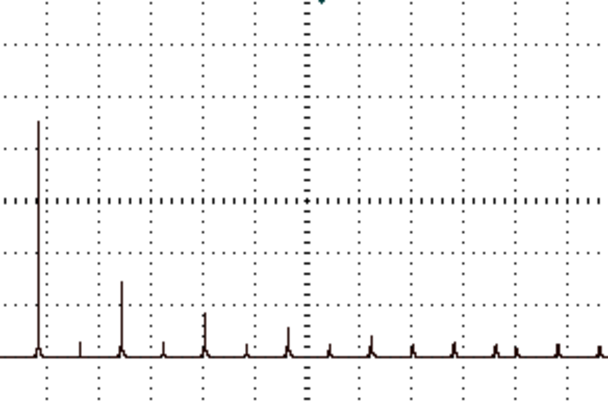
\includegraphics[width=0.7\textwidth]{Bilder/FT_RE2.pdf}		
\caption{Fourieranalyse der Rechteckspannung.}
	\label{fig:FT_RE}
\end{figure}


\begin{figure}
	\centering
		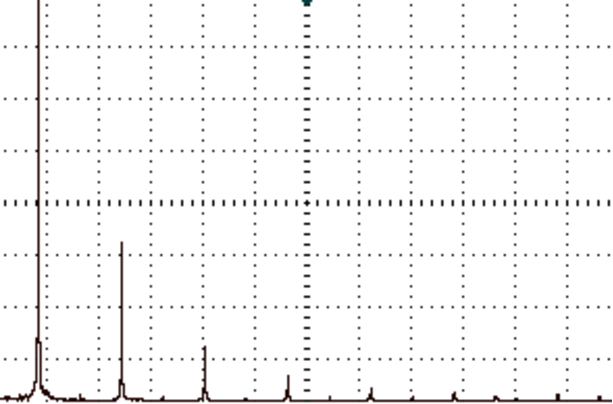
\includegraphics[width=0.7\textwidth]{Bilder/FT_DE2.pdf}		
\caption{Fourieranalyse der Dreieckspannung.}
	\label{fig:FT_DE}
\end{figure}


\begin{figure}
	\centering
		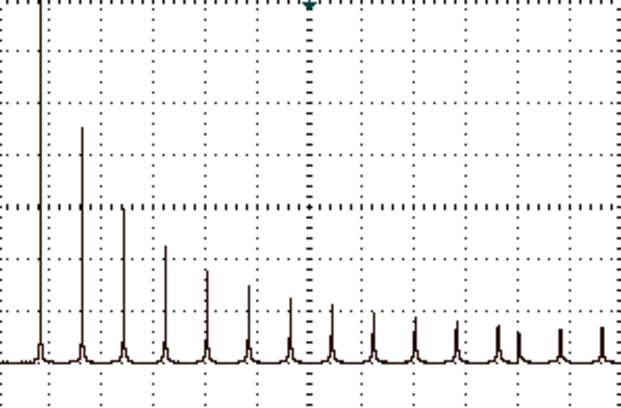
\includegraphics[width=0.7\textwidth]{Bilder/FT_SZ.pdf}		
\caption{Fourieranalyse der Sägezahnspannung.}
	\label{fig:FT_SZ}
\end{figure}

Da Rechteck- und Dreiecksspannug gerade bzw. ungerade Funktionen sind gilt für die Koeffizienten $a_n=0$ bzw. $b_n=0$. Für die in Abbildung \ref{fig:FT_DE} und \ref{fig:FT_RE} dargestellten Amplituden der geraden Koeffizienten gilt $a_n\geqslant0\si\volt$,$b_n\geqslant0\si\volt$, bedingt durch die verwendeten Bauteile in der Messung. Diese Abweichungen lassen sich für größere $n$ nur schwierig von den Amplituden der ungeraden Koeffizienten unterscheiden.

















\subsection{Fouriersynthese}
Bei der Fouriersynthese sollen die in Kapitel \ref{sec:FT} untersuchen Schwingungen aus einzelnen Koeffizienten hergestellt werden. Dazu werden die Amplituden der verschiedenen Oberschwingungen am Oberwellengenerator eingestellt und die Phase so geändert, dass die auf dem Oszilloskopbildschirm dargestellte Summenspannung dem gewählten Spannungsverlauf entspricht. In Tabelle \ref{tab:FS} sind die Amplituden der unterschiedlichen Oberwellen für Rechteck-, Dreieck- und Sägezahnspannung aufgetragen.

\begin{table}
	\centering
	\begin{tabular}{cccc}	
	\toprule
\multicolumn{1}{c}{n} & \multicolumn{3}{c}{$U_n\:/\si{\milli{\volt}}$}\\
	{} & {Rechteck} & {Sägezahn} & {Dreieck}\\
	\midrule
 1 & 634.8  & 634.8  & 634.80\\
 2 &   0    & 318.00 &   0\\
 3 & 216.73 & 212.00 &  70.72\\
 4 &   0    & 159.76 &   0\\
 5 & 130.20 & 127.65 &  25.48\\
 6 &   0    & 106.45 &   0\\
 7 &  92.90 &  91.20 &  13.27\\
 8 &   0    &  79.49 &   0\\
 9 &  72.08 &  70.55 &  7.95\\
	\bottomrule
	\end{tabular}
	\caption{Fouriersynthese drei verschiedener Spannungen.}
	\label{tab:FS}
\end{table}






\begin{figure}
	\centering
		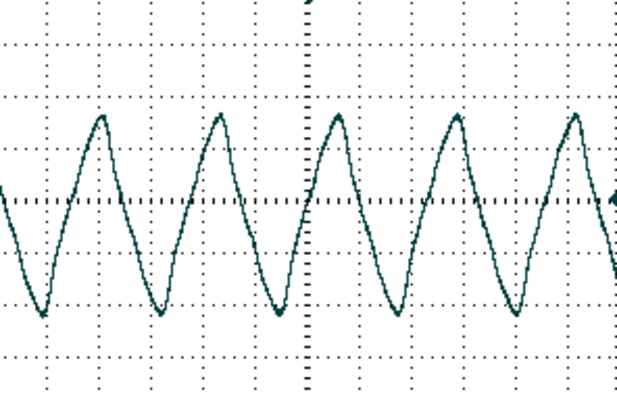
\includegraphics[width=0.7\textwidth]{Bilder/1-9_DE.pdf}		
\caption{Fouriersynthese der Dreiecksspannung.}
	\label{fig:1-9_DE}
\end{figure}






\begin{figure}
	\centering
		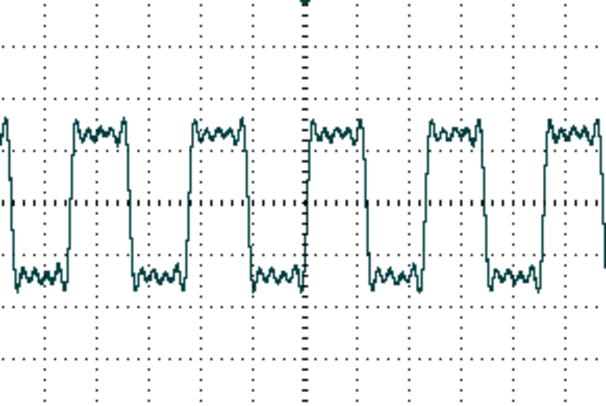
\includegraphics[width=0.7\textwidth]{Bilder/1-9_RE.pdf}		
\caption{Fouriersynthese der Rechteckspannung.}
	\label{fig:1-9_RE}
\end{figure}




\begin{figure}
	\centering
		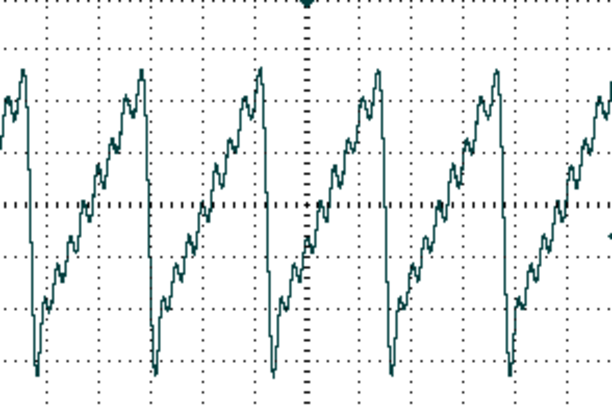
\includegraphics[width=0.7\textwidth]{Bilder/1-9_SZ.pdf}		
\caption{Fouriersynthese der Sägezahnspannung.}
	\label{fig:1-9_SZ}
\end{figure}

